\documentclass{article}
\usepackage{tikz, comment}
\usepackage{pifont}
\usepackage{fontspec}
\usetikzlibrary{arrows, decorations.markings, decorations.pathreplacing}
\begin{comment}
:Title: Not defined yet
:Tags: sohcahtoa;area using polar coordinates, polar integral formula ;sine, sin ;polar form of a complex number;cardioid
:Prob: 0.4705;0.4577;0.437;0.416;0.392
:Author: Prof.Hu Ji-shan, HKUST
:Slug: No name yet

Description Here.........
\end{comment}
\begin{document}\centering

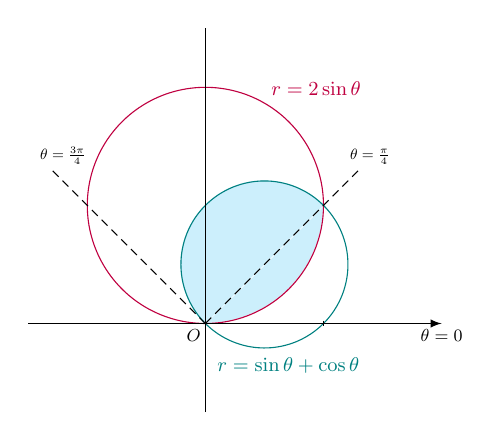
\begin{tikzpicture}[>=latex,xscale=.5*3, yscale=.5*3][font=\sf\small]

%\draw[xstep=1cm,ystep=1cm,color=gray!80] (0, -1) grid (8, 8);

\draw[white, fill=cyan!20, samples=100, smooth, domain=0:pi/4, variable=\t]
plot ({(2*sin(\t r))*cos(\t r)}, {(2*sin(\t r))*sin(\t r)})--(0,0);

\draw[cyan!20, fill=cyan!20, samples=100, smooth, domain=pi/4:3*pi/4, variable=\t]
plot ({(sin(\t r)+cos(\t r))*cos(\t r)}, {(sin(\t r)+cos(\t r))*sin(\t r)})--(0,0);

\draw[purple, samples=100, smooth, domain=0:pi, variable=\t]
plot ({(2*sin(\t r))*cos(\t r)}, {(2*sin(\t r))*sin(\t r)});

\draw[teal, samples=100, smooth, domain=0:pi, variable=\t]
plot ({(sin(\t r)+cos(\t r))*cos(\t r)}, {(sin(\t r)+cos(\t r))*sin(\t r)});

\node[teal, xshift=30, yshift=-15, scale=0.8] at (0,0) {$r=\sin \theta + \cos \theta$};
\node[purple, xshift=40, yshift=85, scale=0.8] at (0,0) {$r=2\sin\theta$};

\draw[densely dashed, samples=100, smooth, domain=0:1.3, variable=\x]
plot ({\x}, {tan((pi/4) r)*(\x)})node[above, xshift=4, scale=0.6] {$\theta = \frac{\pi}{4}$};

\draw[densely dashed, samples=100, smooth, domain=0:-1.3, variable=\x]
plot ({\x}, {tan((3*pi/4) r)*(\x)})node[above, xshift=4, scale=0.6] {$\theta = \frac{3\pi}{4}$};


\foreach \x in {1}
\draw (\x,2pt/3) -- (\x,-2pt/3)
node[anchor=north] {}%{\tiny$\x$}
;
\foreach \x in {}
\draw (\x,2pt/3) -- (\x,-2pt/3)
node[anchor=south] {\tiny$\x$}
;
\foreach \y in {}
\draw (-2pt/3,\y) -- (2pt/3,\y)
node[anchor=east] {}%{\tiny $\y$}
;

\draw[->] (-1.5, 0) -- (2, 0)node[below, scale=0.7] {$\theta=0$};
\draw[] (0, -0.75) -- (0, 2.5);

\node[scale=0.7] at (-0.3/3, -0.3/3) {$O$};

\end{tikzpicture}
\end{document}